\documentclass{article}

\usepackage[ngerman]{babel}
\usepackage{graphicx}
\usepackage{indentfirst}
\usepackage{hyperref}
\usepackage{geometry}
\usepackage{changepage}
\usepackage{booktabs}
\usepackage{float}
\usepackage{tabulary}
\usepackage{multirow}

\graphicspath{ {./images/} }
\setlength\parindent{0pt}

\makeatletter
\newcommand{\sectionauthor}[1]{
	{\parindent 0em \large \scshape Autor: #1 \par \nobreak \vspace*{1em}}
	\@afterheading
}
\newcommand{\specification}[3]{
	{\parindent 0.5em \hangindent 3em \hypertarget{spec:#1:#2}{\textbf{/#1#2/}} #3 \par \nobreak \vspace*{0.5em}}
}
\makeatother

\title{Bibliotheksanwendung - Feinspezifikation}
\date{\today\\v1.0}
\author{
	Ivan Charviakou\\
	León Liehr\\
	Mohamad Najjar\\
	Jonas Picker\\
	Sergei Pravdin
}

\begin{document}
\maketitle
\begin{figure}[h]
	\centering
	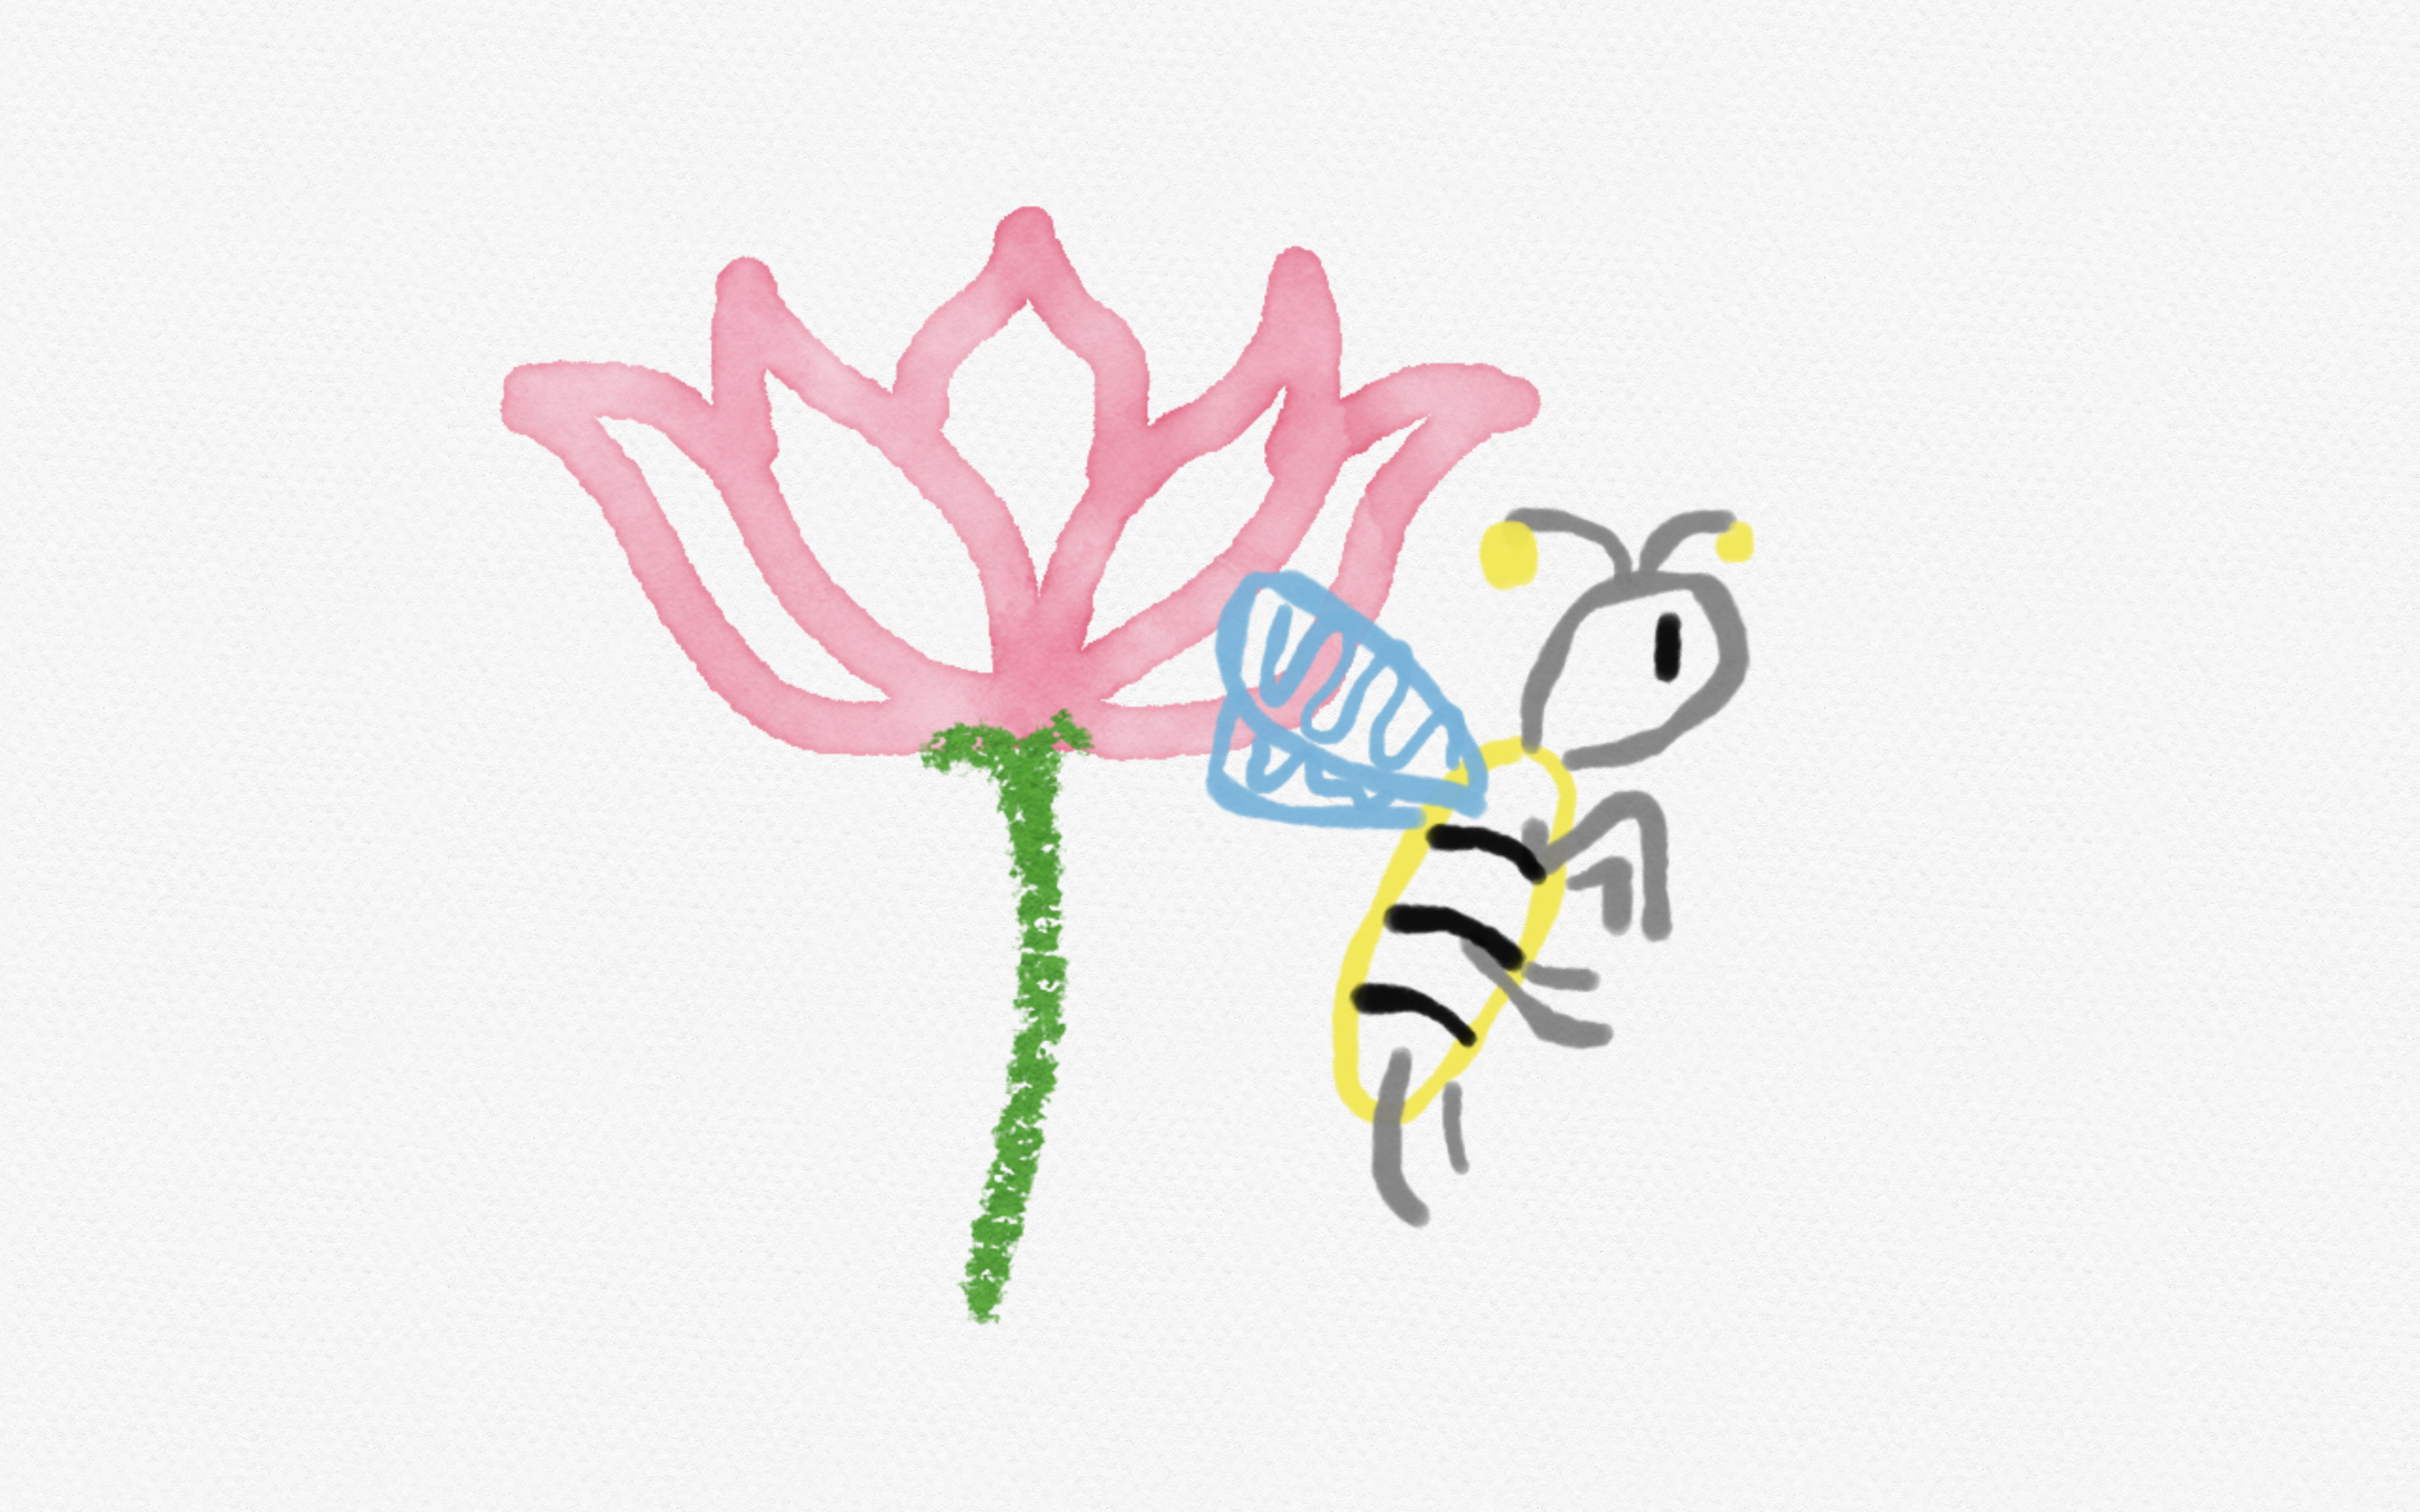
\includegraphics[width = 30em]{Logo}
\end{figure}
\newpage
\tableofcontents
\newpage

%----------------------------------------------------------------------Kapitel 1--------------------------------------------------------------------------------------------

\section{Einleitung}
Bei diesem Dokument handelt es sich um die Feinspezifikation unseres Bibliothekssystems. Es baut direkt auf dem vorangegangenen Entwurf auf und enthält einen noch genaueren Umriss der zu erstellenden Applikation.

%----------------------------------------------------------------------Kapitel 2--------------------------------------------------------------------------------------------

\section{Projektübersicht}
\sectionauthor{Ivan Charviakou}

\subsection{Paketübersicht}
Das folgende Diagramm stellt die MVC-Architektur mit den Beziehungen zwischen den einzelnen Komponenten anhand der gegebenen Applikation dar. 
Dabei folgt die Komponentenaufteilung der Paketstruktur der Applikation und es werden die Paketnamen zusammen mit den wichtigsten darin enthaltenen Klassen / Komponenten / Funktionalitäten angegeben. 
Zudem entsprechen die Farben, die die Pakete im Diagramm besitzen, den Farben im nachfolgenden Klassendiagramm.

\subsection{Ordnerstruktur}
Im Folgenden wird die Ordnerstruktur des Projekts als Ordnerbaum dargestellt. 
Während die Paketstruktur im Ordner 'BiBi.src.main.java' abgebildet ist, enthält 'BiBi.src.main.webapp.view' die verwendeten Facelets mit entsprechender Rollenzuordnung.


%----------------------------------------------------------------------Kapitel 3--------------------------------------------------------------------------------------------


%----------------------------------------------------------------------Kapitel 4--------------------------------------------------------------------------------------------


%----------------------------------------------------------------------Kapitel 5--------------------------------------------------------------------------------------------


%----------------------------------------------------------------------Kapitel 6--------------------------------------------------------------------------------------------


%----------------------------------------------------------------------Kapitel 7--------------------------------------------------------------------------------------------


%----------------------------------------------------------------------Kapitel 8--------------------------------------------------------------------------------------------


%----------------------------------------------------------------------Kapitel 9--------------------------------------------------------------------------------------------


\end{document}